\documentclass[11pt,a4paper]{article}
\usepackage[margin=2.5cm]{geometry}
\usepackage[T1]{fontenc}
\usepackage{amsmath,amssymb,booktabs,graphicx,tabularx,array}
\usepackage[authoryear,round]{natbib}
\usepackage{xurl}
\usepackage{needspace}
\usepackage[colorlinks=true,linkcolor=blue,citecolor=blue,urlcolor=blue]{hyperref}
\graphicspath{{results/}}
\newcommand{\NationalRows}{13652}
\newcommand{\CountryIDs}{236}
\newcommand{\AccountPass}{183}
\newcommand{\AccountFail}{53}
\newcommand{\PilotPass}{8}

\emergencystretch=3em
\title{Ecological assets behind improving accounts:\\a boundary-matched test of composition masking}
\author{Amin Abaee\\\small Independent Researcher, Tehran, Iran\\\small\href{mailto:amin_abaee@ut.ac.ir}{amin\_abaee@ut.ac.ir}\\\small ORCID: \href{https://orcid.org/0000-0002-0019-1842}{0000-0002-0019-1842}}
\date{}
\hypersetup{pdftitle={Ecological assets behind improving accounts: a boundary-matched test of composition masking},pdfauthor={Amin Abaee},pdfkeywords={Ecological Footprint; Biocapacity; Natural capital accounting; Above-ground biomass; Partial identification; Subpixel biomass allocation; Land-use change}}
\begin{document}
\maketitle
\begin{abstract}
Biocapacity accounts and physical ecological assets describe distinct quantities, so agreement between their changes depends on observation boundaries, measurement definitions and uncertainty. This study assesses the compatibility of national biocapacity accounts, forest-cover observations and above-ground woody-biomass products for a forest-led physical comparison. The national account workbook contains \NationalRows\ records across \CountryIDs\ country and territory identifiers; \AccountPass\ identifiers satisfy publication, completeness and numerical-consistency criteria for 2015--2023. All eight countries selected for methodological evaluation satisfy these account criteria. A bounded Brazilian comparison aligns 2015 and 2023 mapped cover with the native biomass grid, distinguishing forest formations, savannas and plantations. Physical comparability additionally requires territorial correspondence, explicit forest definitions, missing-observation treatment and change uncertainty. Examination of biomass product metadata and methods identifies three consequential distinctions: geographic cells are not equal-area observations, aggregated biomass density is expressed per grid-cell rather than forest area, and change-quality classifications are derived from the same endpoint estimates they assess. The design separates extent and density contributions, quantifies spatially offsetting local net changes, and requires reporting comparisons on identical observational support. The results concern account availability, measurement compatibility, local mapped-cover endpoints and conditional biomass-allocation sets; national forest-stock trends, account--asset divergence and conversion associations are not estimated. Within the Brazilian footprint, allocation-only biomass-difference sets contain zero for both mapped-cover groups even when the point maps are treated as exact. The inspected reference artifacts do not provide paired endpoint labels for local change validation.
\end{abstract}

\noindent\textbf{Keywords:} Ecological Footprint; Biocapacity; Natural capital accounting; Above-ground biomass; Partial identification; Subpixel biomass allocation; Land-use change.


\section{Introduction}
Biocapacity is expressed in global hectares, combining physical area with productivity-based factors. Above-ground biomass is a mass of specified living woody material within a geographic support. These quantities are related through ecological production but are not interchangeable measures of ecosystem assets. The distinction between natural-capital stocks and accounting flows has an established basis in the Ecological Footprint literature \citep{Mancini2017}. A quantitative assessment requires separate observation operators and an explicit treatment of their domains.

Composition-dependent land-use models show that transfers towards a land class with a higher annual contribution per hectare can increase a model account while reducing another land class's area \citep{Abaee2026}. Such a mechanism motivates an empirical comparison but does not determine the sign of an observed forest-stock trend. Existing European forest-condition accounting also demonstrates the importance of spatially heterogeneous changes within an aggregate \citep{Maes2023}. Forest condition, extent, biomass and regeneration remain distinct ecological attributes.

\Needspace{15\baselineskip}
The empirical comparison addresses four questions:
\begin{enumerate}
\item How do independently estimated forest extent and above-ground woody biomass change on matched geographic and temporal supports?
\item When national biocapacity increases, do those physical assets increase, decrease or remain unresolved, and how much local change is offset within national totals?
\item Is account--asset divergence associated with independently observed forest-to-cropland conversion after distinguishing harvest, fire, plantation dynamics and regrowth?
\item Does adding independent asset information change an assessment when cases, weights, uncertainty and coverage are held comparable?
\end{enumerate}
The first question establishes the physical outcomes on which the remaining comparisons depend. The sample includes all directions of account and asset change rather than only increasing-account cases. The analysis reported here establishes account availability, screens territorial and observation support, and quantifies mapped cover within a bounded Brazilian footprint; it does not estimate country-level physical changes or conversion associations.

\section{Materials and methods}
\subsection{Sources and observational domains}
The account source is the National Ecological Footprint and Biocapacity Accounts, Edition 2026, results and metadata version 1.0 \citep{Lo2026}. The primary comparison interval is 2015--2023. The secondary comparison domain is 2010--2020, conditional on compatible endpoints and separately justified cross-sensor change uncertainty. Absolute total biocapacity is the principal account measure. Terrestrial, excluding-built-up and forest-component accounts, together with separately labelled per-person values, define alternative account domains. The account's own area fields belong to its input lineage and are not independent physical validation measurements.

The biomass source is ESA Climate Change Initiative Biomass version 7.0 \citep{SantoroCartus2026}. The product provides above-ground woody biomass density estimates for 2005--2012 and 2015--2024. Metadata and coordinate inspection used the nominal 50 km aggregate and the 2010--2020 change product. Product definitions and uncertainty interpretation follow the Product User Guide, Algorithm Theoretical Basis Document, end-to-end uncertainty budget and validation report \citep{PUG2026,ATBD2025,E3UB2025,PVIR2026}. Bounded native-grid observations at 2015 and 2023 distinguish missing, observed-zero and valid values; they do not estimate national coverage or biomass change. The 2010--2020 example describes product structure; it is not a change-validation dataset for the primary interval.

The observation system combines C- and L-band radar retrievals with structural calibration and land-cover-dependent processing. The C-band branch is generated at 150 m spacing and resampled to the 100 m L-band grid. Interannual refinement of merging weights, including land-cover-specific exceptions, improves consistency but does not establish independent endpoint errors or independent 100 m observations. Land-cover information affects calibration, masking of selected classes and merging decisions; the product does not impose a universal forest mask over vegetated land. Published zero estimates are retained separately from missing observations without interpreting them as independent evidence of absent woody vegetation \citep[pp.~57--59, 82--83, 87, 91, 95, 101--102]{ATBD2025}.

Eight countries were selected for evaluation of geographic and measurement compatibility: Brazil, Indonesia, Democratic Republic of the Congo, Cameroon, Canada, Finland, France and Australia. This purposive selection provides environmental and logistical contrasts rather than a probability sample. Country-level account availability and physical observation compatibility are assessed separately. The full set of account identifiers is retained in the availability analysis, irrespective of any expected direction of ecological change.

\subsection{Territorial correspondence and observation support}
Country screening uses the full published geoBoundaries gbOpen ADM0 geometries, identified by fixed repository commits and source hashes \citep{Runfola2020}. Their represented years range from 2016 to 2021; a common geometry across endpoints defines the screening support, not evidence that legal boundaries or account conventions were unchanged. Quantized source geometries with invalid polygon topology are repaired computationally, with the original objects and repair indicators retained. These operations do not certify positional or territorial accuracy.

Polygon areas and their intersections with the native biomass domain, $80^\circ$N to $60^\circ$S, are calculated on WGS84. Geographic linework is densified to at most $0.02^\circ$ before geodesic area calculation to approximate clipped parallels. These polygon areas may contain inland or jurisdictional waters and are not forest-area measurements. Forest support, observed zeros, missing observations and converted land require distinct definitions. ISO identifiers and national account availability do not, by themselves, establish common territorial support for all components, particularly fishing accounts. The Supplementary Information distinguishes geographic domain coverage from valid observations and analytical admission.

\subsection{Account availability and numerical consistency}
Account availability requires a record for every year in 2015--2023, publication flags that permit the relevant biocapacity quantities, and finite, nonnegative required values. Population must be positive. Required fields comprise the five biocapacity components, their total, forest and cropland areas, and population. Flags \texttt{+++}, \texttt{++} and \texttt{+} satisfy the publication criterion; their different trade and consumption detail does not imply a ranking of physical measurement precision. Flags indicating unpublished, missing or estimated-only information do not satisfy the criterion.

The sum of the five published components is compared with the reported total. A tolerance of 3 gha accounts for rounding of five component values and their total. This is a numerical-consistency tolerance, not an ecological threshold. Duplicate country--year keys, missing years and missing required fields are evaluated explicitly. The Supplementary Information specifies the rules and country results.

\subsection{External land-cover support}
The Brazilian support comparison uses MapBiomas Collection 11 annual land-cover and land-use maps at nominal 30 m spacing for 2015 and 2023 \citep{MapBiomas2026}. The footprint is the same geometry-selected $256\times256$ native biomass-cell rectangle used for observation-support assessment; it is not selected using forest cover or biomass changes and is not a national probability sample. Both cover endpoints use the same published collection and geographic grid.

The operational formations group comprises Forest Formation (3), Mangrove (5), Floodable Forest (6) and Wooded Sandbank Vegetation (49). Savanna Formation (4), Flooded Savanna (7) and Forest Plantation (9) remain separately identified. A formations-plus-savanna quantity is reported as a different cover grouping, not an uncertainty interval around the formations target. These mapped classes do not automatically identify all forest land use, temporarily unstocked forest or ecological assets. The official class definitions are biome-specific.

For each native biomass cell, group fractions are calculated from the WGS84 areas of intersections with finer mapped pixels. Geographic spacing is not treated as equal-area sampling, and missing or unclassified support is retained separately rather than renormalized away. Published classifications may incorporate temporal gap filling and filtering, so complete label coverage does not imply a direct, contemporaneous observation at every pixel. The Supplementary Information specifies the area-overlap calculation and observation limits.

\subsection{Physical support and stock decomposition}
For a defined support $\Omega$ and a density referring to that same support, stock is
\[
Q_t=\int_{\Omega} d_t(x)\,\mathrm dA(x),
\]
where $d_t$ is a biomass density with a specified area denominator. Geographic raster cells require latitude-dependent area weights. The computational method integrates meridian--parallel rectangles on the WGS84 ellipsoid; dateline crossings are divided into separate longitude intervals.

For positive forest areas $A_0,A_1$ and compatible stocks $Q_0,Q_1$, let $D_t=Q_t/A_t$. The symmetric decomposition
\begin{align}
\Delta Q_{\mathrm{extent}}&=(A_1-A_0)(D_1+D_0)/2,\label{eq:extent}\\
\Delta Q_{\mathrm{density}}&=(D_1-D_0)(A_1+A_0)/2\label{eq:density}
\end{align}
sums exactly to $Q_1-Q_0$. The contributions describe changes in aggregate area and mean density; they do not identify causal effects. Zero-area endpoints require a separately defined treatment because forest-only density is undefined there. No physical stock decomposition is estimated from the account area fields alone.

\subsection{Conditional within-cell biomass allocation}
Native CCI AGB is a full-pixel density, so a finer mapped group fraction does not allocate biomass within a mixed cell. A conditional allocation calculation holds the published point maps, grid and epochs fixed and allows any nonnegative within-cell biomass distribution, without a finite subcell density cap or temporal allocation constraint. These assumptions define a minimal algebraic model, not a complete ecological or measurement-error model.

Let $q_{it}=A_i\widehat d_{it}$ be the auxiliary full-cell biomass mass, $P_t^g$ the cells entirely mapped as group $g$, and $H_t^g$ all cells with a positive-area intersection with that group. The compatible aggregate allocation set is
\[
\widehat{\mathcal I}_t^g=[L_t^g,U_t^g],\qquad
L_t^g=\sum_{i\in P_t^g}q_{it},\quad U_t^g=\sum_{i\in H_t^g}q_{it}.
\]
Integer counts of intersecting finer pixels determine these categories; no near-zero/near-one ecological fraction threshold is imposed. All cells remain in the target footprint. Using pure cells to anchor the lower bound is not a persistent-pure-only analysis sample. Endpoint sets imply the allocation-difference set $[L_{2023}^g-U_{2015}^g,\,U_{2023}^g-L_{2015}^g]$ under the stated absence of temporal restrictions. The Supplementary Information establishes attainability within this minimal model. The sets are not confidence intervals or guaranteed bounds on true forest biomass: map error, density error, epoch mismatch and additional ecological constraints are not represented.

\subsection{Spatially offsetting local changes}
For local stock changes $\Delta Q_i$ on a common observed support, define
\[
G=\sum_i[\Delta Q_i]_+,\qquad L=\sum_i[-\Delta Q_i]_+,
\]
with net change $G-L$, offset mass $\min(G,L)$ and cancellation fraction
\begin{equation}
K=1-\frac{|G-L|}{G+L},\qquad G+L>0.\label{eq:cancel}
\end{equation}
$K$ is undefined when $G+L=0$. The components are positive and negative local net changes, not gross biological growth, recruitment, mortality or harvest. Their values depend on spatial support and measurement error. Interpretation therefore requires effective-resolution and zero-change error-model assessment. Temporal comparisons require repeated observations at identifiable dates rather than interpolated or model-generated annual independence.

\subsection{Uncertainty, validation and information comparisons}
The relevant error structure includes temporal and spatial covariance, systematic bias, land-transition classification error and incomplete coverage. An assessment of biomass levels does not establish the accuracy of biomass change. Independent forest-to-cropland observations require a justified reference design and transition-specific uncertainty \citep{Olofsson2014}.

CCI's uncertainty model already propagates correlated retrieval errors within annual image stacks and spatially correlated errors in aggregated products. Those terms must be distinguished from cross-year covariance of the final maps. In particular, the L-band within-stack correlation assumption of 0.5 is not an estimate of correlation between the 2015 and 2023 endpoint errors. The uncertainty budget's change-variance expression sums endpoint variances without a cross-year term; this omission does not establish that the true covariance is zero \citep[pp.~14--22, 23--28]{E3UB2025}. Change inference on fixed support requires the joint endpoint covariance structure and the difference of systematic endpoint errors. Uncertainty in forest classification, mixed-cell allocation and observation support remains separate.

Reporting comparisons require common cases and weights, together with coverage estimates for the full eligible population and pairwise overlap. Features derived from the target outcomes are distinguished from independently observed information, and algebraically redundant quantities are identified before interpreting an increment in reporting detail. Diagnostic comparisons require separate calibration and held-out evaluation, with uncertainty in estimated error rates. Practical-change thresholds and classification rules must be fixed without using held-out outcomes. Whole-pipeline calibration must account for spatial support, covariance, systematic bias and incomplete coverage, and comparisons with simple account, endpoint and trend baselines must use the same observations. No classification-performance estimates or physical change-resolution thresholds are inferred from the account availability criteria.

The public CSV, vector and XLSX reference representations linked by MapBiomas are examined separately for endpoint-label completeness, coordinate consistency, sampling-weight fields and explicit training indicators. A geographic reference location is not automatically an independently validated paired observation. Reference coverage is evaluated within the identical fixed Brazilian footprint. Blank reference entries are not interpreted as physical loss or zero biomass.

\section{Results}
\subsection{Availability of national account data}
The workbook contains \NationalRows\ national records, 51 columns and \CountryIDs\ country or territory identifiers spanning 1961--2025. For 2015--2023, \AccountPass\ identifiers satisfy the account availability criteria and \AccountFail\ do not (Figure~\ref{fig:coverage}). All eight selected countries satisfy these criteria. The maximum discrepancy between the component sum and published total within the interval is 2 gha, within the rounding tolerance. These results describe account coverage rather than a physically matched analytical sample.

\begin{figure}[htbp]
\centering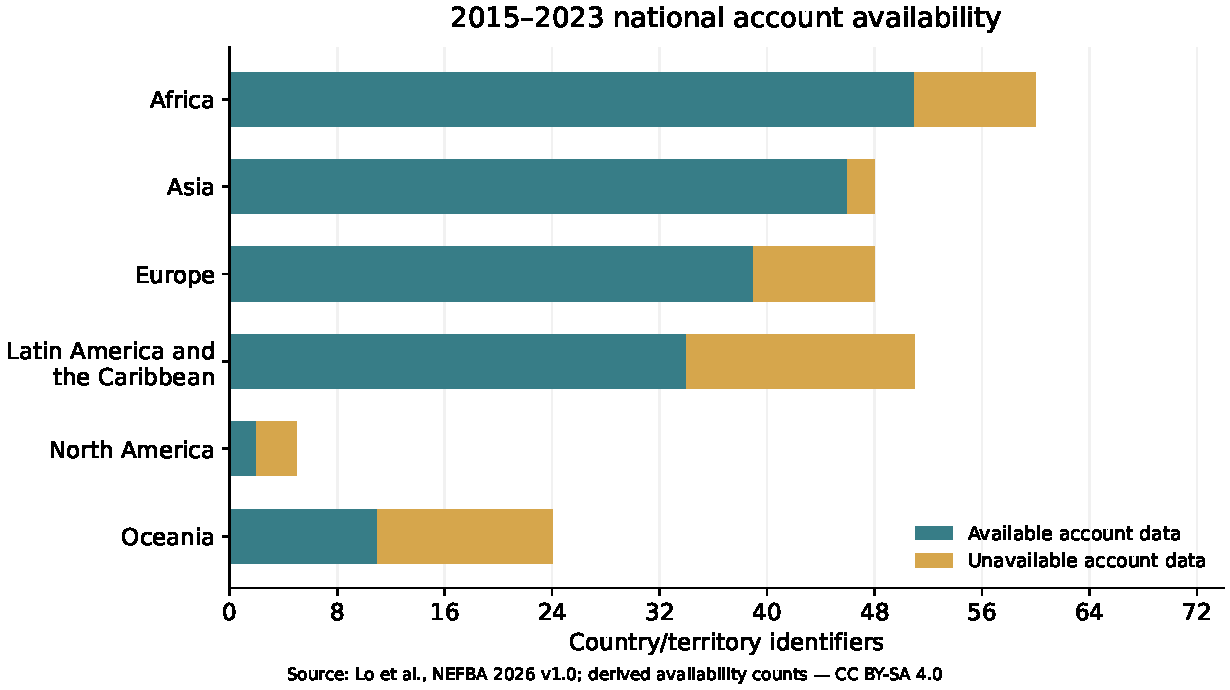
\includegraphics[width=\textwidth]{account_coverage_F06.pdf}
\caption{Availability of national biocapacity account data for 2015--2023 by source UN region. Availability requires complete annual coverage, appropriate publication flags, finite required values and numerical consistency. Data: \citet{Lo2026}; derived availability counts distributed under CC BY-SA 4.0.}\label{fig:coverage}
\end{figure}

\subsection{Territorial and endpoint compatibility}
The candidate Canadian polygon extends to $83.14^\circ$N. Approximately 1.24\% of its polygon area lies north of the biomass product's $80^\circ$N limit; the other seven candidate polygons lie within the documented latitude domain. These are geometric-domain results, not estimates of forest or biomass observation coverage. The biomass or forest content of the omitted Canadian support has not been established and cannot be assumed to be zero.

The French candidate polygon covers metropolitan-European coordinates, while the account workbook lists French Guiana, Guadeloupe, Martinique, R\'eunion and Mayotte separately. The Australian polygon includes outlying components. Both cases require component-specific territorial reconciliation rather than a sovereign-state label alone. The examined Copernicus satellite-land-cover catalogue and retrieval form provide epochs through 2022, not the required 2023 endpoint \citep{CDS2026}. This limitation applies to that product, not to every possible forest observation source. A 2022 classification cannot be substituted for 2023 without changing the comparison and assessing its consequences. No candidate has yet met all territorial, forest-support, complete-coverage and change-validation requirements for analytical admission.

\subsection{Mapped cover on a common Brazilian support}
The fixed footprint has area 61,830.34\,ha and contains $65{,}536$ native biomass cells. Each land-cover subset comprises $846\times845$ finer cells intersecting this rectangle. All target cells have complete published-label coverage at both endpoints under the declared unclassified-code convention. This is classification coverage within the local footprint, not national coverage or evidence that temporal gap filling was unnecessary.

Table~\ref{tab:brazil_cover} distinguishes the mapped quantities. The formations group occupies 6.99\% in 2015 and 7.29\% in 2023; including savannas gives 19.68\% and 18.49\%, respectively. The opposite endpoint directions concern different vegetation groupings and do not establish a resolved ecological change, a preferred forest definition or an account--asset divergence.

\begin{table}[htbp]
\centering\small
\caption{Local mapped-cover endpoints on the identical Brazilian footprint. Values are area-overlap summaries of MapBiomas Collection 11 classifications, not independently validated forest-area estimates. The formations-plus-savanna row overlaps the first row and must not be added to it.}\label{tab:brazil_cover}
\begin{tabular}{lrr}
\toprule
Mapped quantity & 2015 (ha) & 2023 (ha)\\\midrule
Forest formations & 4,319.25 & 4,510.43 \\
Formations plus savanna & 12,169.71 & 11,435.33 \\
Plantation (separate) & 10.66 & 16.91 \\
Open water (separate) & 244.52 & 320.46 \\
\bottomrule
\end{tabular}
\end{table}

There are $13{,}301$ native cells with a nonzero formations fraction at either endpoint and $10{,}385$ at both endpoints, but only $625$ are mapped entirely as formations at both endpoints. Mixed formations cells number $10{,}865$ in 2015 and $11{,}154$ in 2023. These descriptors show the difference between an area fraction and a whole-cell forest selection. Restricting the analysis to persistent pure cells would omit changing and mixed support; that restriction is not used to define a national forest-change sample.

\begin{figure}[htbp]
\centering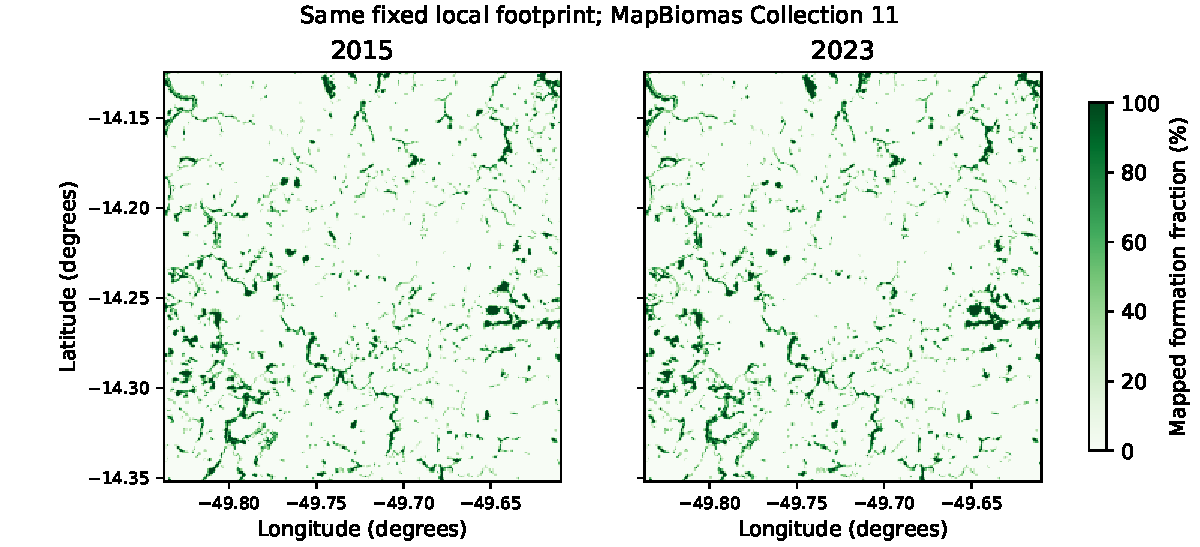
\includegraphics[width=.98\textwidth]{brazil/BRA_F05_support_fractions.pdf}
\caption{Mapped forest-formations fractions within the same fixed local rectangle in 2015 and 2023. Fractions refer to classes 3, 5, 6 and 49; savannas and plantations are separate. The complement includes other vegetation and land uses, not absence of ecological assets. The maps do not estimate biomass change or establish national representativeness. Source: MapBiomas Project, Collection 11; area-overlap processing described in the text.}\label{fig:brazil_support}
\end{figure}

\subsection{Reference coverage and compatibility}
The CSV and vector reference archives each contain $85{,}152$ records but differ in temporal content and representation. The CSV has annual class fields through 2023, with only $4{,}053$ nonblank entries for that endpoint. The vector table ends in 2022. The CSV uses textual class names, whereas the vector table uses numeric class representations; a compatible source-specific crosswalk is required before comparing those labels with Collection 11.

Seven reference locations occur within the fixed Brazilian footprint in each artifact, with coordinates verified against the vector point geometries. All seven CSV 2023 class entries are blank; the vector artifact has no such endpoint field. Neither examined artifact therefore supplies a local paired 2015/2023 reference sample. This is a limitation of these inputs, not evidence of absence of forest or ecological change. Collection 11's documented assessment and other possible reference sources are not invalidated by this finding.

The fully examined XLSX representation contains the same $85{,}152$ identifiers as the CSV. At every identifier, all 117 common annual class, interpreter-count and border fields match after whitespace, Unicode and integral-number serialization normalization. Coordinates and training-role tokens also match. The workbook therefore adds neither a new local paired-endpoint sample nor an independent reference replication.

The CSV explicitly marks $9{,}999$ records as training samples. The remaining $75{,}153$ are not thereby certified independent evaluation observations. Interpretation provenance, possible sample reuse, appropriate class/transition labels and probability-design treatment remain required. The Supplementary Information details coordinate-attribute and weight-field discrepancies that also preclude uncritical pooling of the artifacts.

\subsection{Biomass support and uncertainty definitions}
The inspected biomass aggregate contains 18 epochs on a $720\times360$ longitude--latitude grid with $0.5^\circ$ spacing. The nominal 50 km designation does not imply equal-area cells. The Product User Guide defines aggregated density per total grid-cell area; it does not define a forest-area-normalized density. Its aggregate uncertainty calculation includes a spatial covariance component \citep{PUG2026}. Native biomass values likewise refer to full pixels and are not forest-masked. Consequently, the density denominator, valid-data support and uncertainty interpretation must be specified before a forest stock can be estimated. A finer mapped forest fraction does not identify the share of whole-pixel biomass inside that fraction.

The change product includes density difference, change standard deviation and quality-class layers. Quality classes are derived from the endpoint estimates and their uncertainty intervals, with additional growth-limit and spatial-filtering operations. The inspected example calculation of change standard deviation uses the sum of endpoint variances without a temporal covariance term. These classes therefore contain information about the processing rule and its inputs; they are not independent reference observations or calibrated 95\% confidence statements. Supplementary Tables S2--S3 give the source definitions and associated interpretation requirements.

CCI's v7 stock validation includes the primary endpoint years and uses plot and LiDAR reference data reported as withheld from map production \citep[pp.~11--14, 64, 67]{PVIR2026}. Reference preparation includes growth-rate adjustment for temporal mismatches of up to ten years and forest-fraction harmonization of small plots \citep[p.~18]{PVIR2026}. These stock comparisons provide relevant evidence about the observation system, but epoch-specific reference counts are not counts of paired change observations. The reported standard-error layer represents random error; the variance-consistency diagnostic does not estimate confidence-interval coverage for the local forest-stock difference \citep[p.~19]{PVIR2026}.

\subsection{Conditional biomass-allocation sets}
Table~\ref{tab:allocation} reports the local allocation sets for the same two mapped groups. Both endpoint-difference sets contain zero, permitting negative, zero and positive differences under the minimal allocation model. Thus the sign is not identified by these point maps and nonnegativity alone, before considering measurement uncertainty. Adding savannas changes the mapped domain rather than supplying a confidence interval for the formations target.

\begin{table}[htbp]
\centering\small
\caption{Conditional allocation sets in the fixed Brazilian footprint, in $10^3$ Mg of above-ground woody biomass. Published cover and biomass point maps are treated as exact. Entries are compatible allocations under nonnegativity and unrestricted component density, not statistical confidence intervals or validated forest-stock changes.}\label{tab:allocation}
\begin{tabular}{lrrr}
\toprule
Mapped domain & 2015 & 2023 & 2023 minus 2015\\\midrule
Formations & $[44.23, 279.19]$ & $[55.22, 326.23]$ & $[-223.97, 282.00]$ \\
Formations + savanna & $[229.75, 434.47]$ & $[256.36, 489.29]$ & $[-178.11, 259.53]$ \\
\bottomrule
\end{tabular}
\end{table}

The auxiliary sum of full-cell masses is $463.92\times10^3$ Mg in 2015 and $529.16\times10^3$ Mg in 2023. These totals refer to every native cell in the local rectangle, not only mapped forest; their increase does not identify a forest-specific gain and does not replace the primary forest-stock target. Observed zero-density cells remain included. The formations group has 791 and 876 mapped-pure cells at the two endpoints, with mixed cells retained in the upper sets. No within-forest mean-density point estimate or extent--density decomposition is inferred from these allocation sets.

\section{Discussion}
The account coverage supports a multi-country comparison, but availability alone does not establish matched physical support. The distinction is consequential where country definitions, forest masks, mapped observation domains or density denominators differ. Whole-cell biomass averages and forest-only means require different area multipliers. Applying the same multiplier to both would change the physical quantity being estimated.

Spatial compensation also requires measurement-specific interpretation. Opposing local net changes can occur within an increasing national total, but spatial error can produce the same pattern in point estimates. Cancellation must therefore be evaluated with spatial covariance, resolution and zero-change error models. A diagnostic evaluated against a target-derived quality class would measure agreement with that processing rule, rather than independently verified ecological change.

The evidence comprises account availability, geographic-domain screening, local mapped-cover endpoints, conditional allocation sets, product definitions and the analytical design. It does not estimate national forest-stock trends, account--asset divergence, conversion associations or reporting-rule accuracy. National inference requires territorial and mask reconciliation, independently justified change uncertainty, and coverage-sensitive treatment of missing or converted pixels. Soil, wetlands and fisheries involve different observation domains and are outside the present assessment.

The Brazilian example separates mapped forest formations, savannas and plantations rather than treating all woody vegetation as one invariant target. Temporal filters and gap filling can affect endpoint timing, while map-wide classification accuracy does not determine local or transition accuracy. The public reference-point downloads inspected are labelled Collection 9; compatibility with Collection 11, sample reuse, design weights and transition-specific reference interpretation require assessment before change validation. Different map publishers do not establish independent errors, particularly where auxiliary information or reference data may overlap.

The biomass observation operator imposes a further distinction. Even an exactly known forest fraction does not allocate total woody biomass between forest and other parts of a mixed pixel. A whole-territory woody-biomass stock is a different estimand from forest-only stock; neither should be relabelled as the other. Extent--density decomposition requires the stock and forest-area operands to describe the same support. No forest-only biomass estimate is obtained by multiplying native density by mapped forest fraction. The computed allocation sets quantify one part of the identification problem while conditioning on uncertain point maps; they do not supply a calibrated change-resolution rule.

The provider validation and the present identification limits address different questions. A held-out stock comparison can assess map agreement on its reference support without identifying forest-specific biomass inside a mixed cell or calibrating a paired 2015--2023 change on the present footprint. The described validation screening excludes plots deforested between inventory and map dates, and temporal harmonization uses growth assumptions; transferring its error characteristics to converted land requires evidence beyond agreement among retained forest observations \citep[pp.~13, 18--19]{PVIR2026}. Reference measurement error, geolocation and within-pixel sampling also contribute to map--reference discrepancies. Accordingly, neither RMSD nor a globally pooled bias pattern is adopted as a local change-error model, and the absence of such a model here is not a claim that the v7 stock product lacks validation.

\section{Conclusions}
National biocapacity data for 2015--2023 satisfy the specified availability criteria for \AccountPass\ of \CountryIDs\ country and territory identifiers. Physical account--asset comparison additionally requires aligned boundaries, the correct biomass area denominator, covariance-aware change uncertainty and independent reference information. The extent--density and spatial-cancellation estimands provide explicit quantities for that comparison while preserving distinctions among accounts, stocks, condition and biological flows. In the local Brazilian example, both mapped-group biomass-difference sets contain zero under the stated minimal allocation model, so that model does not identify a direction of group-specific change.

\section*{Data and code availability}
Source datasets are cited in the text. Derived account-availability tables, source definitions, file hashes and computational methods are available at \url{https://github.com/MIKEAA2020/general-sustainability/tree/main/batch%209/agent%202/ecomod_empirical_followup/F09}. NEFBA-derived tables and figures are distributed under CC BY-SA 4.0. Boundary inputs and boundary-derived data retain their separately documented source licences and attribution requirements. Conditional allocation summaries and topological intersection counts are also supplied; raw native-density arrays are not redistributed. MapBiomas-derived cover summaries identify Collection 11 and the processing used; the provider permits public use with source attribution. Raw country land-cover images, biomass files and provider technical reports are not redistributed.

\section*{Declaration of generative AI in scientific writing}
\href{http://Arena.ai}{Arena.ai} Agent Mode was used to assist with computational methods and literature review.

\begin{thebibliography}{99}
\bibitem[Abaee(2026)]{Abaee2026} Abaee, A. (2026). A rising biocapacity total can mask ecological-capital land drawdown: a two-land model. Manuscript. \url{https://github.com/MIKEAA2020/general-sustainability/tree/main/batch%209/agent%202/ecomod_c17}.
\bibitem[Mancini et al.(2017)]{Mancini2017} Mancini, M. S., Galli, A., Niccolucci, V., Lin, D., Hanscom, L., Wackernagel, M., Bastianoni, S., and Marchettini, N. (2017). Stocks and flows of natural capital: Implications for Ecological Footprint. \emph{Ecological Indicators}, 77, 123--128. \url{https://doi.org/10.1016/j.ecolind.2017.01.033}.
\bibitem[Maes et al.(2023)]{Maes2023} Maes, J., Bruz\'on, A. G., Barredo, J. I., Vallecillo, S., Vogt, P., Rivero, I. M., and Santos-Mart\'in, F. (2023). Accounting for forest condition in Europe based on an international statistical standard. \emph{Nature Communications}, 14, 3723. \url{https://doi.org/10.1038/s41467-023-39434-0}.
\bibitem[Olofsson et al.(2014)]{Olofsson2014} Olofsson, P., Foody, G. M., Herold, M., Stehman, S. V., Woodcock, C. E., and Wulder, M. A. (2014). Good practices for estimating area and assessing accuracy of land change. \emph{Remote Sensing of Environment}, 148, 42--57. \url{https://doi.org/10.1016/j.rse.2014.02.015}.
\bibitem[Lo et al.(2026)]{Lo2026} Lo, K., Basnet, N., Miller, E., Srikanthalingam, B., Foley, B., Van Berkum, J. L., Long, A. H., Toneva, P., Ermina, M., and Klinkenberg, C. (2026). \emph{National Ecological Footprint and Biocapacity Accounts, Edition 2026 (1961--2025): Results and metadata, version 1.0}. Footprint Data Foundation. \url{https://footprint.info.yorku.ca/data/}.
\bibitem[Santoro and Cartus(2026)]{SantoroCartus2026} Santoro, M., and Cartus, O. (2026). ESA Biomass Climate Change Initiative: Global datasets of forest above-ground biomass for 2005--2012 and 2015--2024, v7.0. CEDA. \url{https://doi.org/10.5285/6429d1aafe1e43b9b414e4a5a7f8b903}.
\bibitem[CCI Biomass(2026)]{PUG2026} CCI Biomass (2026). \emph{Product User Guide v7.0}. 19 March 2026. \url{https://climate.esa.int/en/projects/biomass/key-documents/}.
\bibitem[Runfola et al.(2020)]{Runfola2020} Runfola, D., et al. (2020). geoBoundaries: A global database of political administrative boundaries. \emph{PLOS ONE}, 15, e0231866. \url{https://doi.org/10.1371/journal.pone.0231866}. Country-specific geometry sources, represented years and commits: \url{https://www.geoboundaries.org/api.html}.
\bibitem[Copernicus Climate Change Service(2026)]{CDS2026} Copernicus Climate Change Service (2026). \emph{Land cover classification gridded maps from 1992 to present derived from satellite observations}. Catalogue and retrieval form accessed 29 October 2026. \url{https://doi.org/10.24381/cds.006f2c9a}.
\bibitem[MapBiomas Project(2026)]{MapBiomas2026} MapBiomas Project (2026). \emph{Collection 11 of the Annual Land Cover and Land Use Maps of Brazil}. General Algorithm Theoretical Basis Document, class codes and descriptions, and biome appendices. Accessed 29 October 2026. \url{https://brasil.mapbiomas.org/downloads/}.
\bibitem[CCI Biomass(2025a)]{ATBD2025} CCI Biomass (2025a). \emph{Algorithm Theoretical Basis Document, v7.0}. 17 December 2025. \url{https://climate.esa.int/media/documents/Algorithm_Theoretical_Basis_Document_ATBD_V7.0.pdf}.
\bibitem[CCI Biomass(2025b)]{E3UB2025} CCI Biomass (2025b). \emph{End to End ECV Uncertainty Budget, v7.0}. 17 December 2025. \url{https://climate.esa.int/documents/3354/End-to-End_ECV_Uncertainty_Budget_E3B_V7.0.pdf}.
\bibitem[CCI Biomass(2026b)]{PVIR2026} CCI Biomass (2026b). \emph{Product Validation and Intercomparison Report, v7.0}. 24 April 2026. \url{https://climate.esa.int/documents/3356/Product_Validation_Intercomparison_Report_PVIR_V7.0.pdf}.
\end{thebibliography}
\end{document}
